%!TEX root = ../main.tex
\section{Introduction} 
\label{sec:intro}

Data scarcity, which refers to a situation where there is an insufficient amount or quality of training data available to build an accurate and robust machine learning model, can negatively impact the performance and generalization of machine learning models and lead to poor predictions or classifications.

Data scarcity can manifest in two common cases. First, there may not be enough high-quality unlabeled data due to factors such as high costs of data collection, lack of access to relevant data sources, or data privacy and security constraints. Second, annotating unlabeled data can be a time-consuming and expensive process, even if enough high-quality data has been collected.

In the literature, various methods have been utilized to obtain high-quality (unlabeled) data, including data augmentation~\cite{}, data synthesis~\cite{}, and data acquisition~\cite{}.
Once this unlabeled data is collected, it can be labeled using human-labeling methods like crowdsourcing~\cite{} or expert sourcing~\cite{}, or using machine-labeling methods like semi-supervised learning~\cite{} and weak supervision~\cite{}.

Despite all efforts to collect, generate, and label data, a common phenomenon in machine learning is distribution shift, where the distribution of the train data differs from the distribution of the test data in downstream applications.


\stitle{Problem.}
Our main research question in this paper is how to \textit{generate sufficient high-quality unlabeled data that is relevant to downstream applications} and label it using inexpensive and automatic methods such as semi-supervised learning and weak supervision.

A positive answer to this question is crucial as it can help alleviate data scarcity in machine learning with minimal human cost.


\stitle{Challenges.}
\nan{Add after we have the technical sections.}


\stitle{Our Proposal.}
Our main idea is to train a generative model and then iteratively adapt it to the downstream application.
More specifically, \nan{Add more details later, including how XXX can be used to train the generative model and how reinforcement learning can be used to adapt it to the downstream application. These details will be explained at a conceptual level to ensure that readers can understand.}

\stitle{Contributions.}
Our contributions are summarized as follows:

\be
	\item 
	\item 
	\item \nan{If we can have a good summary of experiments, we can either add here or use a ``stitle'' section to highlight the empirical findings.}
\ee

\stitle{Roadmap.}

\begin{figure*}
	\centering
	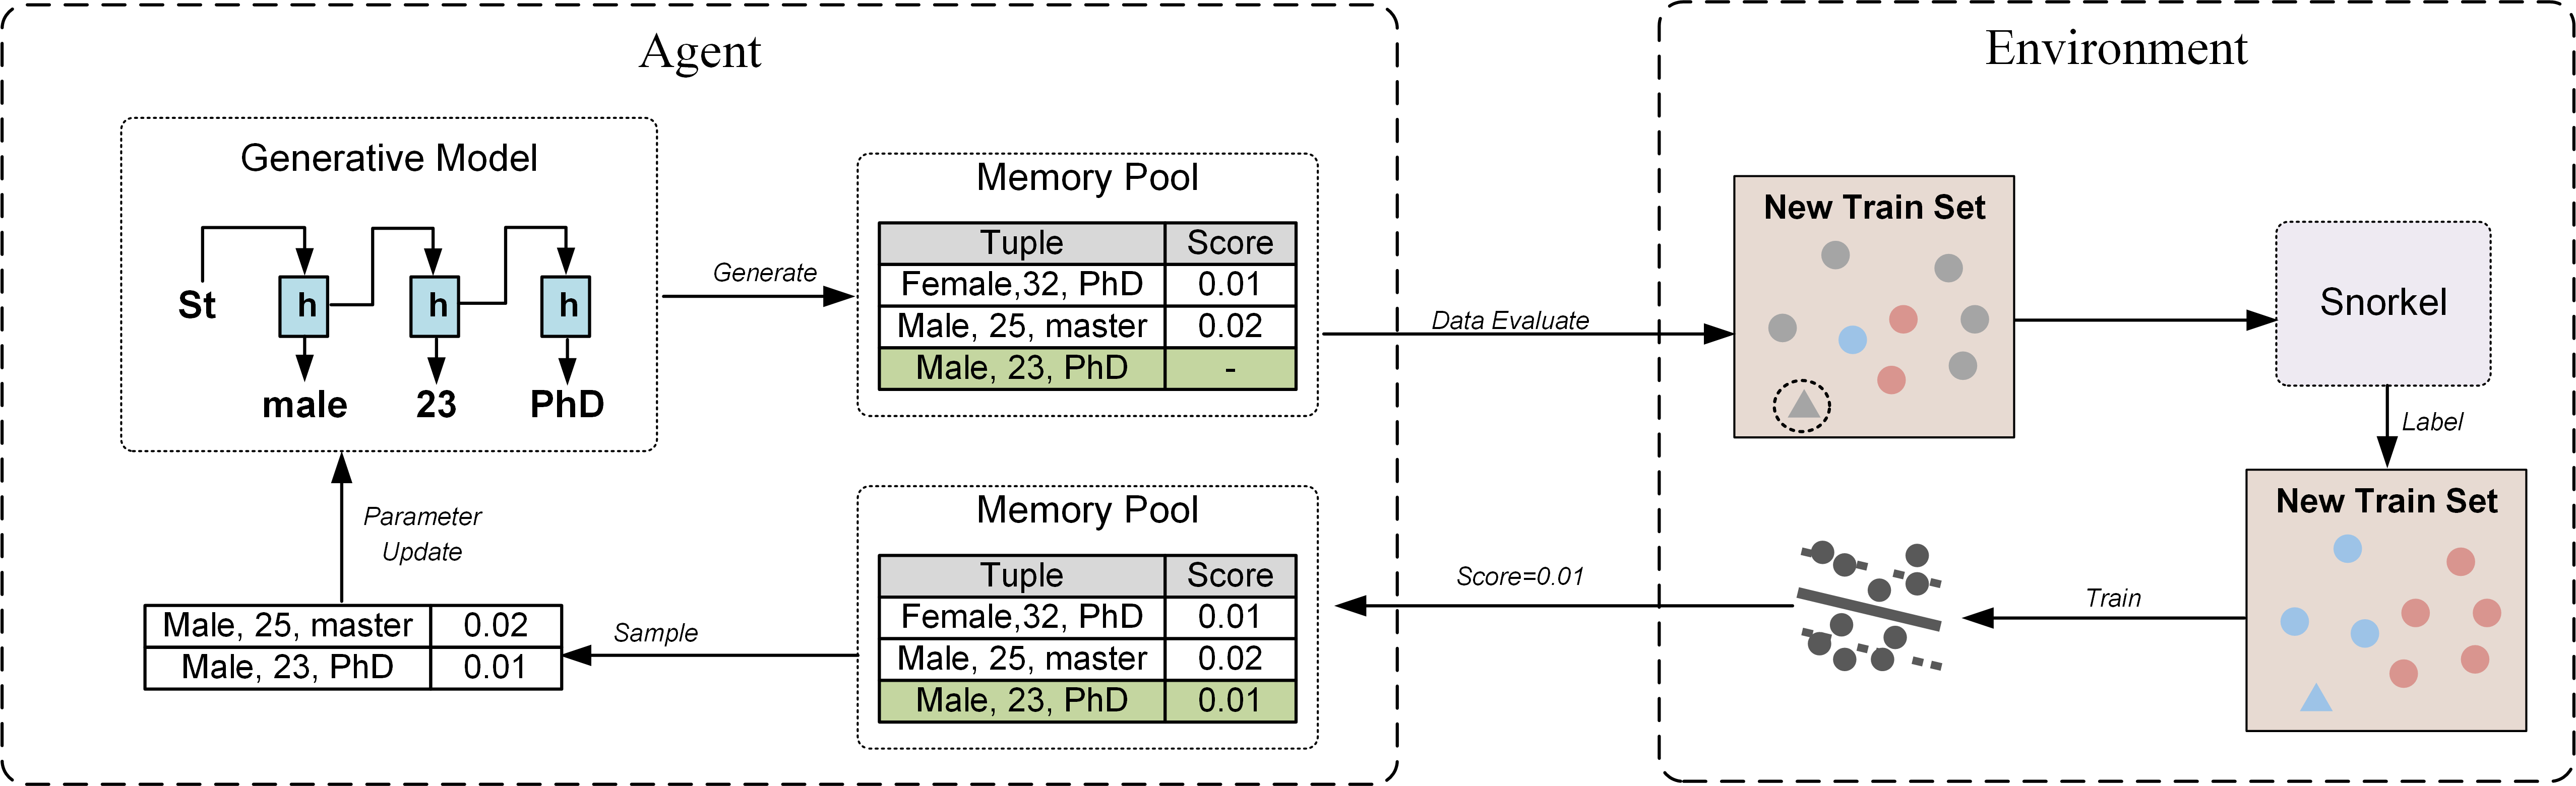
\includegraphics[width=\textwidth]{figures/overview.png}
	\caption{Framework}
	\label{fig:framework}
\end{figure*}

% \begin{itemize}
% 	\item The difference between traditional data generation and ours (for ML model).
% 	\item (Challenge) The key challenges of this problem: learn the generative model from feedback; how to evaluate generated tuples.
% \end{itemize}